Subbab~\ref{sec:verif_fusi_traversability} menjelaskan bahwa nilai traversability efektif yang digunakan oleh pengendali fuzzy dibentuk melalui operasi $\tau_{eff} = \min(\tau_{LiDAR}, \tau_{thermal})$, dengan $\tau_{LiDAR}$ adalah skor koridor yang dihitung dari jarak dinding kiri dan kanan pada jendela sudut lateral robot, dan $\tau_{thermal}$ adalah nilai traversability hasil segmentasi semantik kamera termal setelah melalui tapis lolos-rendah asimetrik. Pada pengujian yang telah dipaparkan pada Subbab~4.3 hingga 4.7, ketiga nilai tersebut dihitung secara internal oleh planner APF namun belum ditampilkan secara eksplisit. Subbab ini memaparkan hasil instrumentasi tambahan yang dilakukan untuk memverifikasi bahwa mekanisme fusi tersebut bekerja sesuai rancangan.

\subsection{Metode Verifikasi}

Untuk memperoleh bukti empiris atas proses fusi, dilakukan penambahan publisher pada node APF yang memancarkan nilai $\tau_{LiDAR}$, $\tau_{thermal}$, dan $\tau_{eff}$ secara bersamaan setiap kali fungsi perhitungan traversability dipanggil. Nilai tersebut kemudian dicatat oleh node pencatat data pada resolusi waktu yang sama dengan siklus kontrol fuzzy ($\pm$10~Hz). Pencatatan dilakukan pada satu trial representatif untuk setiap skenario yang menggunakan mode fuzzy, yaitu S5 (ruang terbuka), S6 (obstacle tunggal), S7 (multi-obstacle statis dengan kucing), dan S8 (multi-obstacle dinamis dengan kucing). Mekanisme fusi hanya aktif pada mode fuzzy sehingga verifikasi ini tidak dilakukan pada skenario baseline (S1--S4).

\subsection{Hasil pada Skenario S7}

Skenario S7 dipilih sebagai kasus utama karena memuat obstacle berprofil rendah (kucing) yang berada pada area \textit{blind-spot} LiDAR sekaligus obstacle statis lain di sepanjang jalur robot. Gambar~\ref{fig:trav_fusion_s7} menunjukkan nilai $\tau_{LiDAR}$, $\tau_{thermal}$, dan $\tau_{eff}$ sepanjang durasi trial, beserta jarak Euclidean antara robot dan kucing pada waktu yang sama.

\begin{figure}[H]
\centering
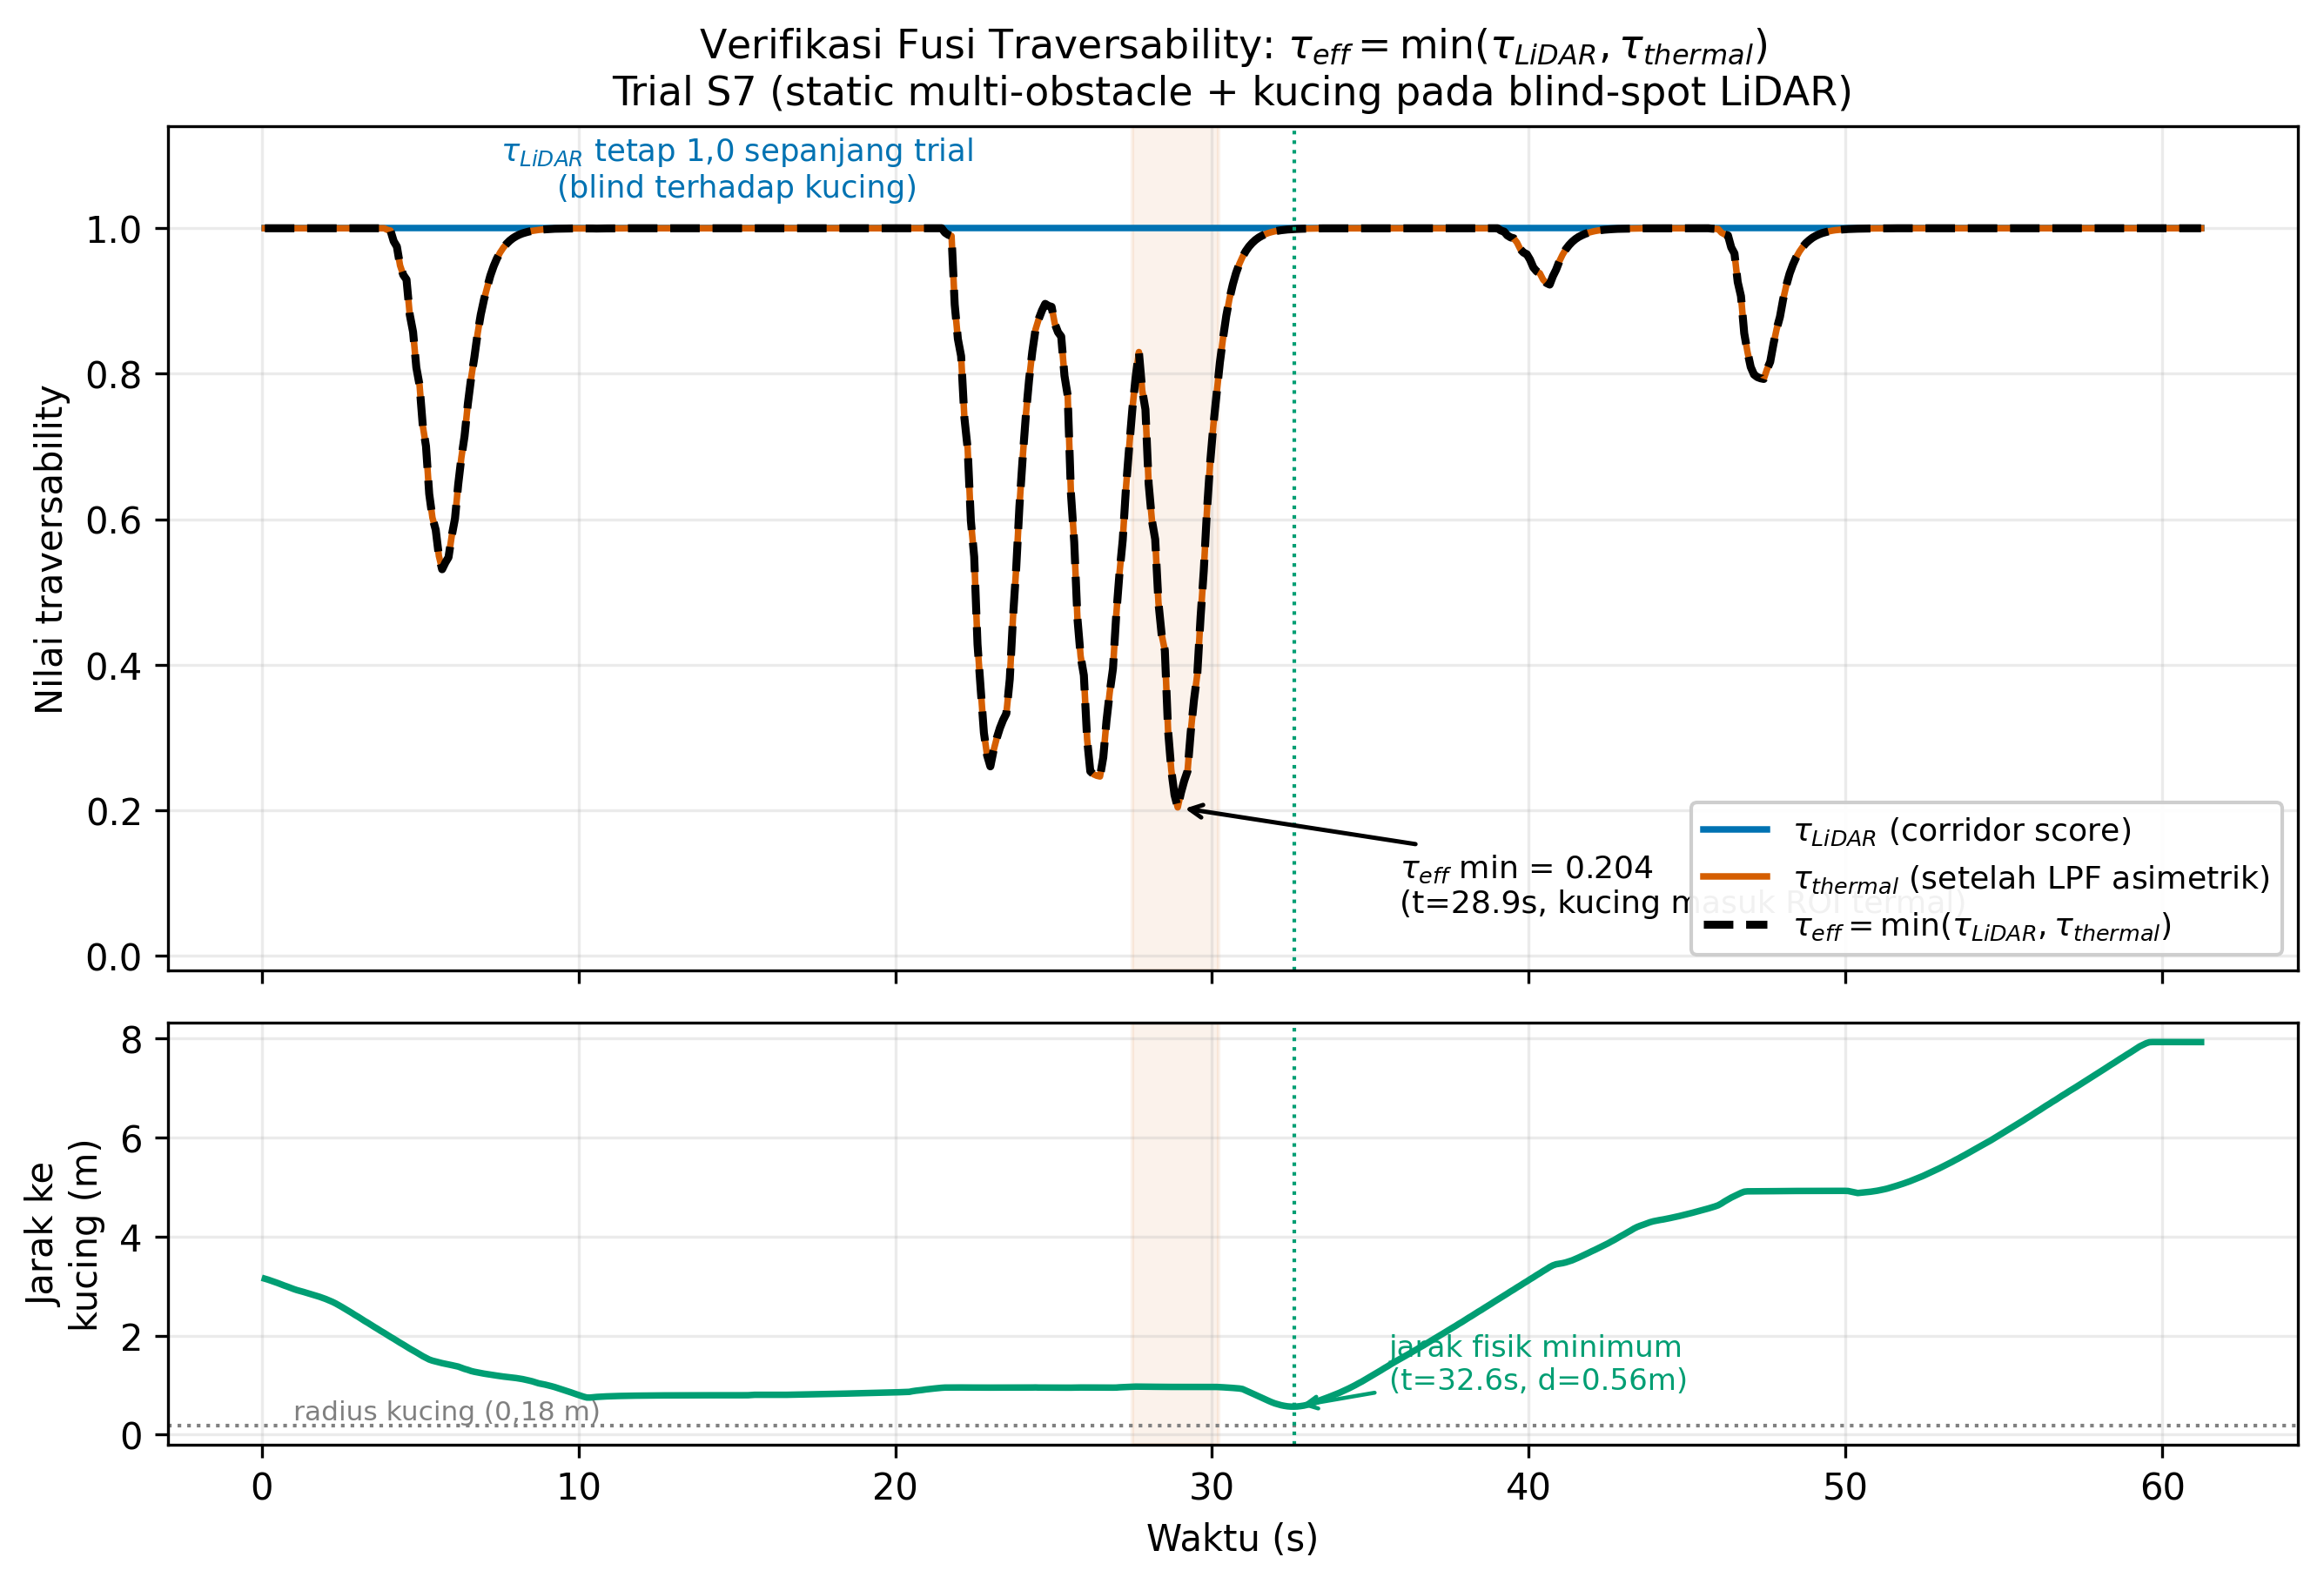
\includegraphics[width=\textwidth]{gambar/fig_trav_fusion_s7.png}
\caption{Nilai $\tau_{LiDAR}$, $\tau_{thermal}$, dan $\tau_{eff}$ terhadap waktu pada trial representatif skenario S7, disertai jarak robot terhadap obstacle kucing.}
\label{fig:trav_fusion_s7}
\end{figure}

Hasil pengujian menunjukkan bahwa $\tau_{LiDAR}$ bernilai konstan 1,0 sepanjang seluruh durasi trial, mengonfirmasi secara empiris bahwa LiDAR tidak memperoleh informasi apa pun mengenai keberadaan kucing, sesuai dengan permasalahan \textit{blind-spot} yang menjadi dasar penelitian ini. Sebaliknya, $\tau_{thermal}$ mengalami penurunan tajam hingga mencapai nilai minimum 0,204 pada detik ke-28,9, bertepatan dengan masuknya kucing ke area ROI kamera termal. Karena $\tau_{eff}$ merupakan hasil operasi minimum dari kedua nilai tersebut, penurunan pada $\tau_{thermal}$ langsung tercermin pada $\tau_{eff}$ tanpa tertahan oleh $\tau_{LiDAR}$ yang tetap tinggi.

Grafik jarak pada bagian bawah Gambar~\ref{fig:trav_fusion_s7} memperlihatkan bahwa titik minimum $\tau_{eff}$ (detik ke-28,9) terjadi lebih awal dibandingkan titik jarak fisik terdekat robot terhadap kucing (detik ke-32,6 dengan jarak 0,56~m). Hal ini terjadi karena kamera termal mendeteksi kucing berdasarkan posisinya di dalam bidang pandang ROI trapesium, bukan semata-mata berdasarkan jarak Euclidean, sehingga sistem dapat memberikan respons yang bersifat antisipatif sebelum jarak robot terhadap obstacle benar-benar mepet.

\subsection{Konsistensi Pola pada Skenario S5--S8}

Untuk menilai apakah pola pada Subbab 4.8.2 bersifat konsisten atau spesifik pada satu trial, verifikasi yang sama dilakukan pada ketiga skenario fuzzy lainnya. Gambar~\ref{fig:trav_fusion_comparison} menam\-pilkan perbandingan $\tau_{LiDAR}$, $\tau_{thermal}$, dan $\tau_{eff}$ pada keempat skenario, sedangkan Tabel~\ref{tab:trav_fusion_summary} merangkum nilai minimum dan maksimum masing-masing komponen.

\begin{figure}[H]
\centering
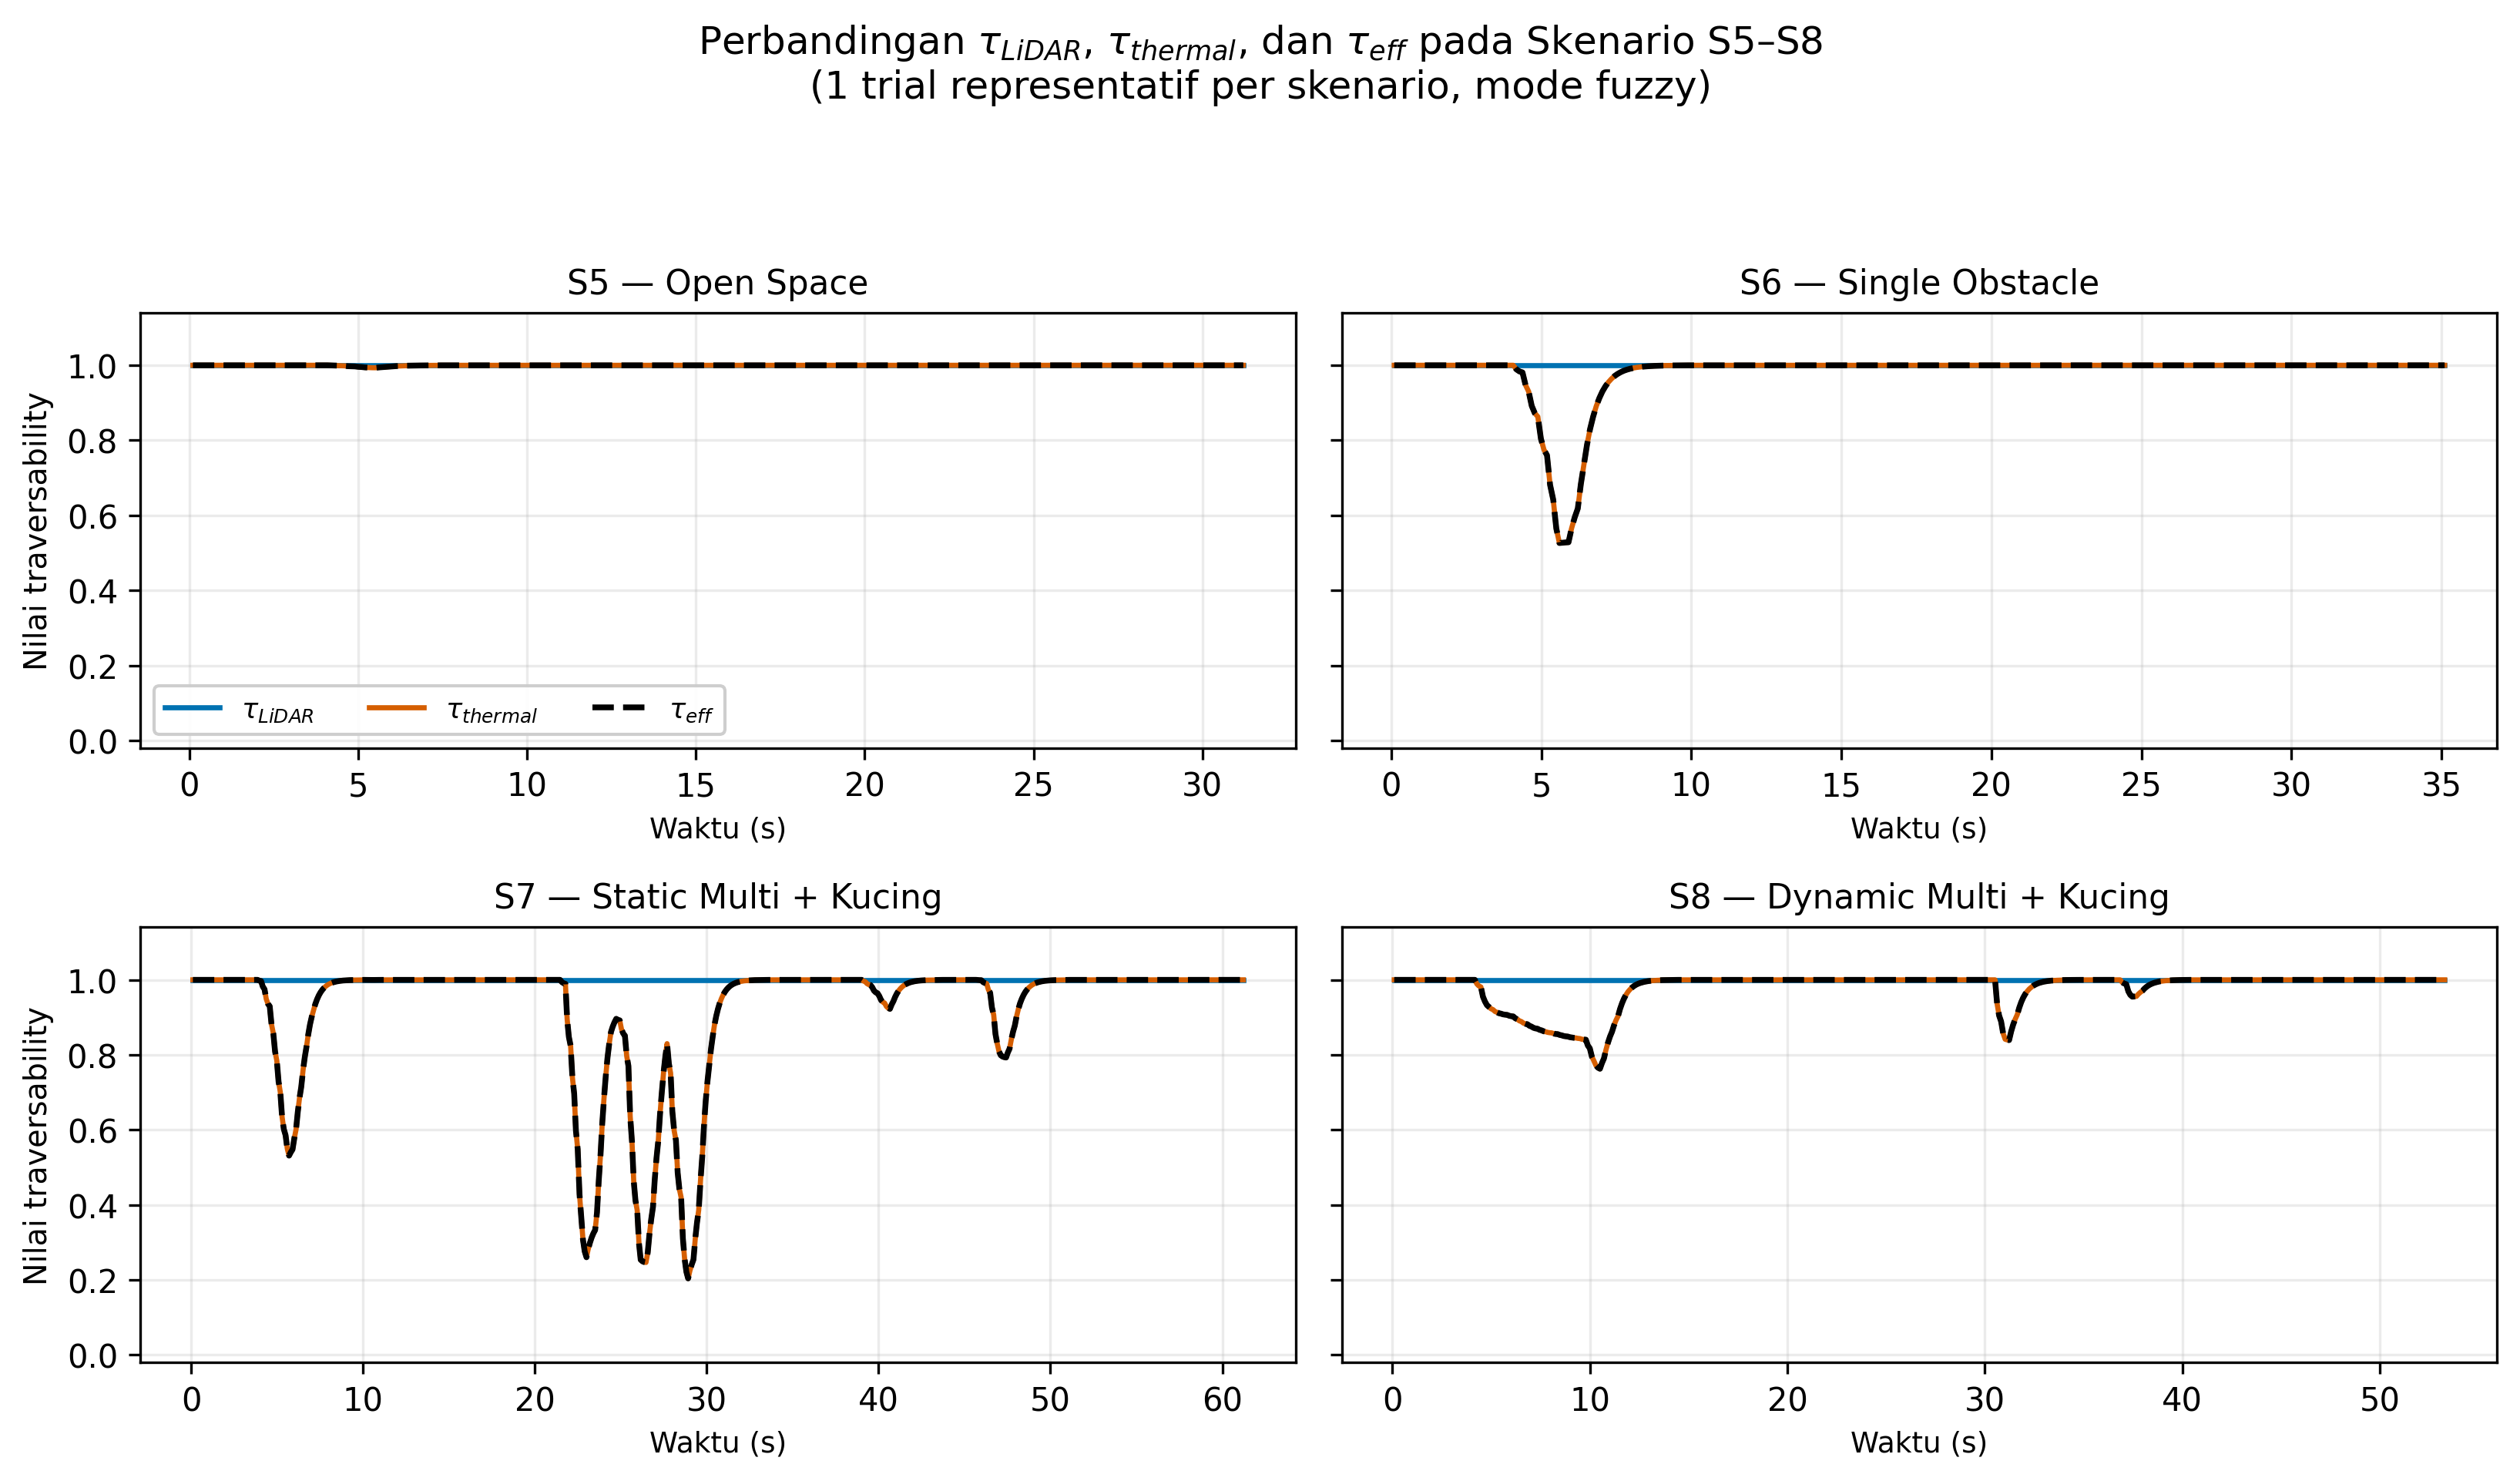
\includegraphics[width=\textwidth]{gambar/fig_trav_fusion_comparison.png}
\caption{Perbandingan $\tau_{LiDAR}$, $\tau_{thermal}$, dan $\tau_{eff}$ pada satu trial representatif untuk skenario S5, S6, S7, dan S8.}
\label{fig:trav_fusion_comparison}
\end{figure}

\begin{table}[H]
\centering
\caption{Ringkasan nilai $\tau_{LiDAR}$, $\tau_{thermal}$, dan $\tau_{eff}$ pada trial representatif skenario S5--S8.}
\label{tab:trav_fusion_summary}
\begin{tabular}{lcccc}
\toprule
Skenario & Kondisi & $\tau_{LiDAR}$ & $\tau_{thermal}$ min & $\tau_{eff}$ min \\
\midrule
S5 & Ruang terbuka          & 1,000 (konstan) & 0,993 & 0,993 \\
S6 & Obstacle tunggal       & 1,000 (konstan) & 0,526 & 0,526 \\
S7 & Multi-statis + kucing  & 1,000 (konstan) & 0,204 & 0,204 \\
S8 & Multi-dinamis + kucing & 1,000 (konstan) & 0,763 & 0,763 \\
\bottomrule
\end{tabular}
\end{table}

Tabel~\ref{tab:trav_fusion_summary} menunjukkan bahwa $\tau_{LiDAR}$ bernilai konstan 1,0 pada seluruh empat skenario yang diuji, sedangkan $\tau_{thermal}$ mengalami penurunan dengan kedalaman yang bervariasi sesuai kompleksitas skenario, dari hampir tidak berubah pada S5 (kontrol negatif tanpa obstacle) hingga penurunan tajam pada S7. Pada seluruh skenario tersebut, $\tau_{eff}$ selalu identik dengan $\tau_{thermal}$ karena operasi $\min(\cdot)$ selalu memilih nilai yang lebih rendah.

Temuan ini perlu dimaknai secara tepat. Konsistennya nilai $\tau_{LiDAR}$ pada 1,0 tidak menunjukkan kegagalan mekanisme fusi, melainkan mencerminkan karakteristik metrik $\tau_{LiDAR}$ itu sendiri. Nilai tersebut dihitung melalui

\begin{equation}
\tau_{LiDAR} = \text{clip}\left(\frac{(d_{kiri} + d_{kanan}) - w_{robot}}{c_{full}},\ 0,\ 1\right)
\end{equation}

dengan $d_{kiri}$ dan $d_{kanan}$ adalah jarak terdekat ke dinding pada jendela sudut lateral robot ($55^\circ$ hingga $125^\circ$), $w_{robot} = 0,55$~m adalah lebar fisik robot, dan $c_{full} = 0,25$~m adalah ambang clearance yang dianggap sudah merepresentasikan kondisi lorong yang sepenuhnya layak dilalui. Berdasarkan formula tersebut, $\tau_{LiDAR}$ baru mulai turun dari 1,0 apabila $d_{kiri} + d_{kanan} < 0,80$~m, yaitu ketika lebar lorong efektif menyempit hingga kurang dari 80~cm.

Gambar~\ref{fig:peta_s3_s7} memperlihatkan kondisi lingkungan pengujian pada skenario S3/S7, yang merepresentasikan tata letak seluruh skenario multi-obstacle pada penelitian ini. Robot bergerak pada area terbuka yang luas, sedangkan dinding penyusun ruangan berada pada jarak yang jauh dari lintasan robot. Obstacle uji (kucing, manusia, dan obstacle statis) ditempatkan sebagai entitas diskret yang melayang pada ruang terbuka tersebut, bukan sebagai penyempit lorong di antara dua dinding. Akibatnya, jendela sudut lateral $55^\circ$--$125^\circ$ yang digunakan untuk menghitung $d_{kiri}$ dan $d_{kanan}$ hampir selalu mengarah ke ruang kosong yang jauh melebihi ambang 0,80~m, sehingga $\tau_{LiDAR}$ senantiasa berada pada nilai tersaturasi 1,0 di sepanjang lintasan.

\begin{figure}[H]
\centering
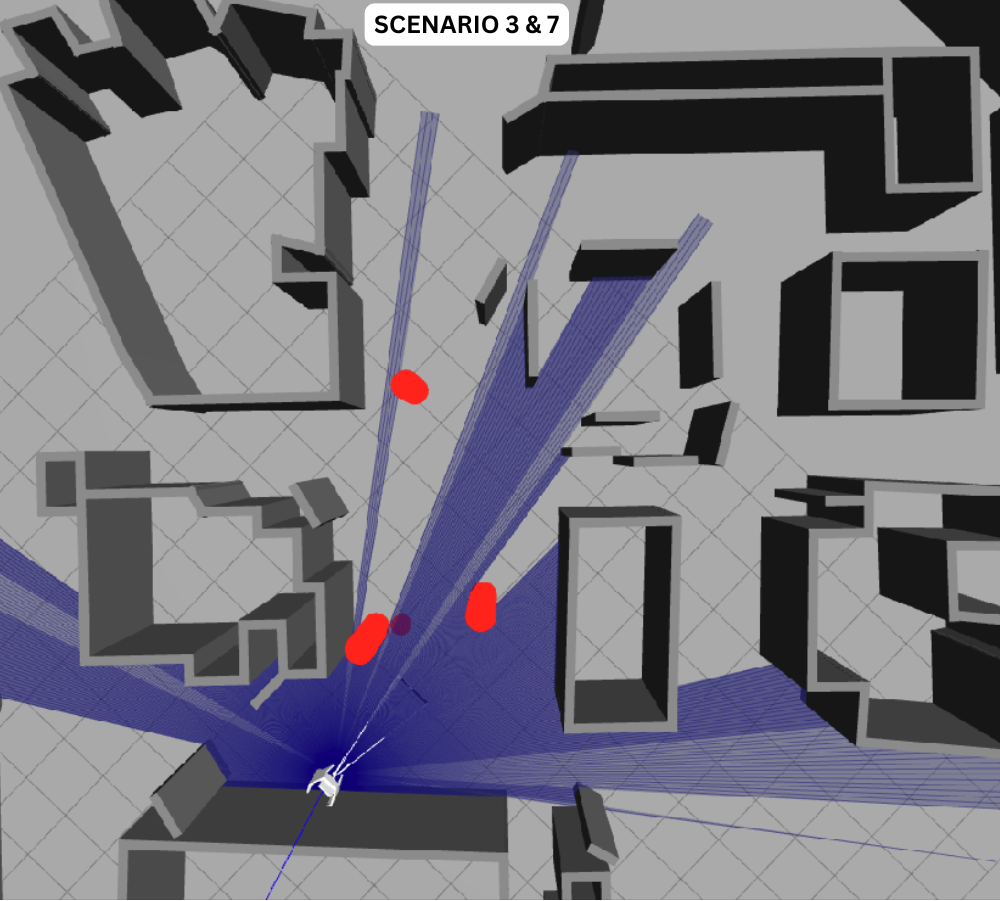
\includegraphics[width=0.5\textwidth]{gambar/3.8_skenario_S3_S7.png}
\caption{Kondisi lingkungan pengujian pada skenario S3/S7 di Gazebo. Obstacle uji (blob merah) berada sebagai entitas diskret pada ruang terbuka, sedangkan dinding penyusun ruangan berada jauh dari lintasan robot.}
\label{fig:peta_s3_s7}
\end{figure}

Seluruh obstacle uji pada penelitian ini, yaitu kucing, manusia, dan obstacle statis, berupa entitas diskret yang berada pada jalur robot dan ditangani melalui gaya tolak terpisah ($F_{rep}$ dan $F_{cat}$), bukan melalui penyempitan lorong yang terukur oleh $\tau_{LiDAR}$. Dengan demikian, operasi $\tau_{eff} = \min(\tau_{LiDAR}, \tau_{thermal})$ tetap terverifikasi bekerja sesuai rancangan, dan pada kondisi lingkungan pengujian ini, $\tau_{thermal}$ secara konsisten menjadi komponen pembatas yang menentukan nilai $\tau_{eff}$.

Hasil ini sekaligus memperkuat urgensi integrasi kamera termal yang menjadi dasar RM1 penelitian ini: pada keempat skenario yang diuji, tidak satu pun momen ditemukan pada rentang waktu tersebut mekanisme berbasis LiDAR mengalami penurunan yang berarti terhadap keberadaan obstacle uji sehingga apabila sistem hanya mengandalkan $\tau_{LiDAR}$, seluruh obstacle pada penelitian ini akan luput dari deteksi traversability. Sebagai catatan keterbatasan, pengujian pada peta dengan segmen koridor sempit diperlukan pada penelitian lanjutan untuk memverifikasi kontribusi $\tau_{LiDAR}$ secara lebih menyeluruh pada kondisi yang benar-benar menyempitkan ruang gerak lateral robot.

\subsection{Implikasi terhadap Masalah \textit{Blind-Spot} LiDAR}

Berdasarkan hasil pada Subbab 4.8.2 dan 4.8.3, dapat disimpulkan bahwa mekanisme pembentukan dan penggabungan traversability yang dirumuskan pada Subbab~\ref{sec:verif_fusi_traversability} telah berhasil diimplementasikan dan diverifikasi secara empiris. Traversability berbasis LiDAR dan traversability berbasis kamera termal keduanya dihitung secara independen pada setiap siklus kontrol, kemudian digabungkan melalui operasi minimum untuk menghasilkan representasi tunggal kondisi lingkungan yang digunakan oleh pengendali fuzzy. Pada seluruh skenario pengujian, mekanisme ini secara konsisten meneruskan kondisi terburuk dari kedua sensor, dengan kamera termal berperan sebagai komponen yang secara konsisten menentukan nilai akhir traversability efektif akibat karakteristik obstacle uji yang bersifat diskret dan berada pada area \textit{blind-spot} LiDAR.